\documentclass{article}
\usepackage{graphicx}
\usepackage{caption}
\usepackage[T1]{fontenc}


\begin{document} % > Compilar con PDFLaTeX
	Consideremos ahora el paralelepípedo
	\begin{figure}[h!] % Ambiente ’figure’
		\centering % imagen sin escalar
		\includegraphics{images/figura3.pdf}
		\caption{Un paralelepípedo}\label{figura3}
	\end{figure}
	Ahora consideremos el sólido $Q$...
	\begin{center} % Escalada a 4cm de ancho
		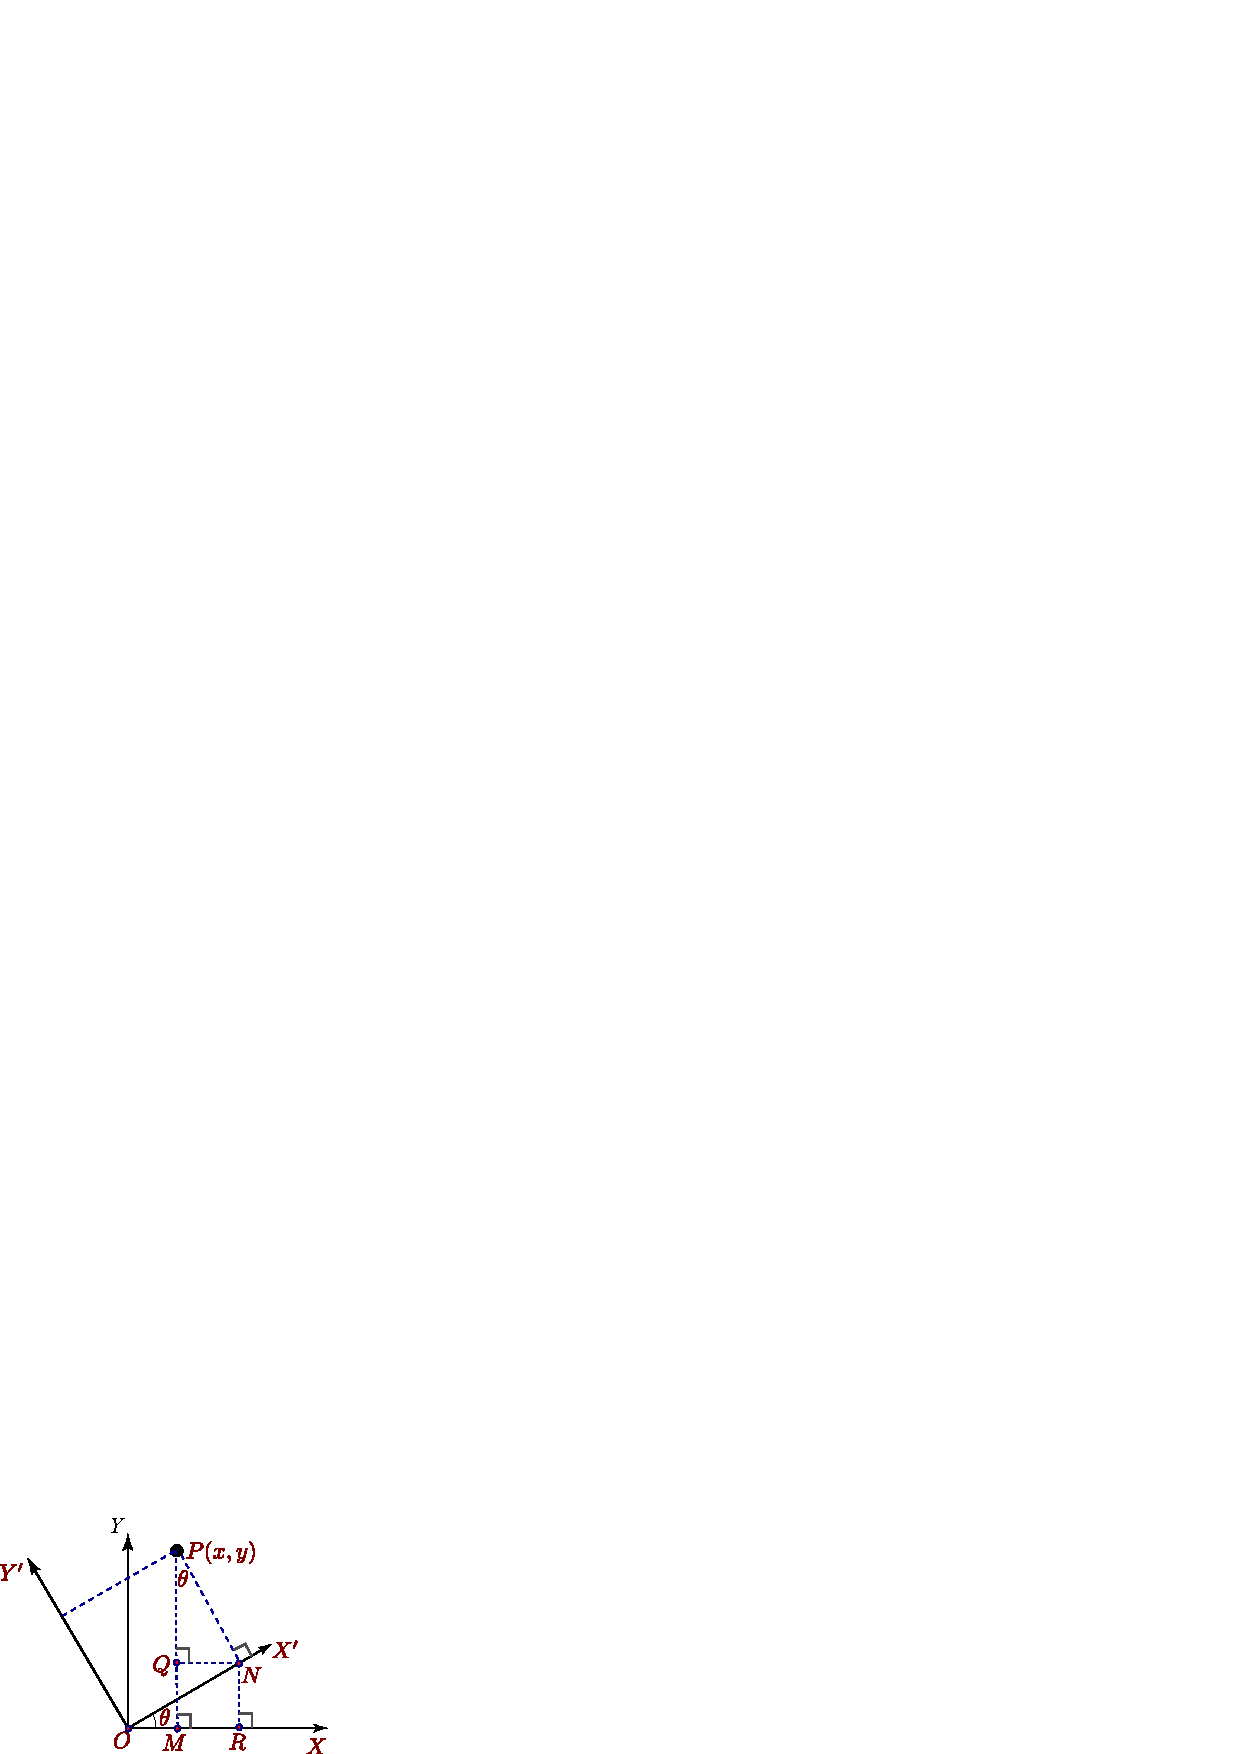
\includegraphics[width =5cm]{images/figura4.pdf}
		\captionof{figure}{Sólido $Q$}
		\label{figura3a}
	\end{center}
\end{document}

